%%%% ijcai17.tex

%\typeout{IJCAI-17 Instructions for Authors}

% These are the instructions for authors for IJCAI-17.
% They are the same as the ones for IJCAI-11 with superficical wording
%   changes only.

\documentclass{article}
% The file ijcai17.sty is the style file for IJCAI-17 (same as ijcai07.sty).
\usepackage{ijcai17}

\usepackage[authoryear]{natbib}
\usepackage[titletoc,toc,title]{appendix}

% Use the postscript times font!
\usepackage{times}

% the following package is optional:
%\usepackage{latexsym} 

% Following comment is from ijcai97-submit.tex:
% The preparation of these files was supported by Schlumberger Palo Alto
% Research, AT\&T Bell Laboratories, and Morgan Kaufmann Publishers.
% Shirley Jowell, of Morgan Kaufmann Publishers, and Peter F.
% Patel-Schneider, of AT\&T Bell Laboratories collaborated on their
% preparation.

% These instructions can be modified and used in other conferences as long
% as credit to the authors and supporting agencies is retained, this notice
% is not changed, and further modification or reuse is not restricted.
% Neither Shirley Jowell nor Peter F. Patel-Schneider can be listed as
% contacts for providing assistance without their prior permission.

% To use for other conferences, change references to files and the
% conference appropriate and use other authors, contacts, publishers, and
% organizations.
% Also change the deadline and address for returning papers and the length and
% page charge instructions.
% Put where the files are available in the appropriate places.

\usepackage{amssymb}
\usepackage{amsthm}
\usepackage{amsmath}
\usepackage{algorithm}
\usepackage[noend]{algpseudocode}
\usepackage{float}
\usepackage[titletoc,toc,title]{appendix}
\usepackage{fixltx2e}
\usepackage{dblfloatfix}
\usepackage{subcaption}
\usepackage{multirow}
\usepackage{ctable}

\usepackage{graphicx}

\raggedbottom %nicer enumerate
\theoremstyle{definition}
\newtheorem{defn}{Definition}[section]

\title{Recursive Feature Generation for Knowledge-based Induction}
%\author{\name Lior Friedman \email liorf@cs.technion.ac.il \\
%	\name Shaul Markovitch \email shaulm@cs.technion.ac.il \\
%	\addr Technion-Israel Institute of Technology\\
%	Haifa 32000, Israel
%}
%\author{Lior Friedman \and Shaul Markovitch\\
%	Computer Science Department \\
%	Technion-Israel Institute of Technology\\
%	Haifa 32000, Israel\\
%	\{liorf,shaulm\}@cs.technion.ac.il}
%\author{Paper ID 661 \\
%		Content Areas: Machine Learning, Feature Generation, Semantic Web, Natural Language Processing
%	}
%TODO: hide for draft. put topics instead
\author{Paper ID 661 \\
		Content Areas: Machine Learning, Feature Selection/Construction, Knowledge-based Learning
	}

\begin{document}
	
\maketitle
	
\begin{abstract}
	Induction algorithms have steadily improved over the years, resulting in powerful methods for learning. However, these algorithms are constrained to using knowledge within the supplied feature vectors. %In recent years, a large collection of both general and domain-specific knowledge bases have become increasingly available on the web. The natural question is how these knowledge bases can be exploited by existing induction algorithms.
	In this work we propose a novel supervised algorithm for injecting external knowledge into induction algorithms using feature generation. Given a feature, the algorithm defines a new learning task over its set of values, and uses the knowledge base to then solve the constructed learning task. The resulting classifier is then used to create new features for the original problem.
	We have applied our algorithm to the domain of text categorization, using large semantic knowledge bases such as Freebase. We have shown that generated features significantly improve the performance of existing induction algorithms.
\end{abstract}

\section{Introduction}
\label{sec:Intro}
In recent decades, we have seen an increasing prevalence of machine learning techniques used in a wide variety of fields. %such as medical diagnosis, vision, and biology.
Most of these methods rely on the inductive approach: given a set of labelled examples, they attempt to locate a hypothesis that is heavily supported by the known data. These methods have proven themselves successful in cases where there is a sufficient number of examples, and a collection of good,
distinguishing features is available.
In many real-world applications, however, the given set of features is not sufficient for inducing a high quality classifier.

One approach for overcoming the difficulty resulting from an insufficiently expressive set of features, is to generate new features based on existing ones. 
These feature generation approaches attempt to combine the given feature set in an effort to create better, more discriminatory features with regards to the induction problem at hand. As an example of this, the LFC algorithm \citep{ragavan1993complex} combines binary features through the use of logical operators such as $\land ,\lnot$.

These feature generation methods all provide us with ways to enhance the performance of induction algorithms through intelligent combinations of existing features. While this approach often suffices, there are many cases where merely combining existing features is not sufficient. 
In such cases, we require knowledge external to the problem in order to solve it effectively.
%Supposed, for example, that the induction problem at hand is to identify people at risk of the genetic disorder Tay-Sachs\footnote{A recessive genetic disorder prevalent mostly among Ashkenazi Jews}. The training set contains examples of people that have developed Tay-Sachs, and examples of people that did not. Since the concept is related to a patient's country of origin, a human expert might look at surnames of former patients, and using his background knowledge regarding surnames, he would link past patient surnames to geographical locations corresponding to high risk, allowing him to identify potential patients with high accuracy.
%A machine learning algorithm, on the other hand, would do poorly, as it lacks the external knowledge required to make that link.

%One known method of utilizing external knowledge is known as Deductive Learning \citep{mitchell1982generalization,dejong1986explanation}. This school of learning methods uses a knowledge base of logical assertions in order to locate a small set of logical conditions that capture the target concept based on examples from that concept. This approach does so using deduction, rather than induction, as its main tool, allowing us to leverage a logical knowledge base effectively.
%There are two main concerns that must be addressed for deductive learning to be effective:
%\begin{enumerate}
%	\item Extensive knowledge bases comprised of logical assertions are difficult to find and create.
%	\item This approach forfeits the progress and power gained by the use of well-known and extensively researched inductive methods.
%\end{enumerate}

%In order to combat these issues, we can make use of the extensive relational knowledge bases that have been constructed as part of the Semantic Web project (see survey, \cite{bizer2009linkedfull}). 
In recent years, extensive relational knowledge bases have gained increasing popularity. These knowledge bases contain facts regarding type-annotated entities covering a multitude of domains. % that are connected via semantically meaningful relations.
 Thus, the question is how relational knowledge can be used to enhance existing induction methods.
There have been several efforts in utilizing Linked Data for unsupervised feature generation. \cite{cheng2011automatedfull} devised a general framework for constructing features from linked data. %By using intelligent queries, it is possible to construct features that utilize the knowledge base in a meaningful way. 
\cite{paulheim2012unsupervisedfull} developed FeGeLOD, an automated, fully unsupervised framework that constructs features by locating and expanding upon entities using relations within the Semantic Web \citep[see][]{bizer2009linkedfull}.%using entity recognition techniques to locate entities and expand upon them using relations within the Semantic Web. % semantically meaningful features in the data set, and expand upon those entities using relations within the Semantic Web. %They then use feature selection techniques to remove features with a large percentage of missing, identical, or unique\footnote{Values which only appear in a single example} values.

In this work, we build upon these existing approaches in order to present a new supervised methodology for generating complex features based on a relational knowledge base. Our algorithm recursively constructs new learning problems from existing feature values, then uses knowledge bases to construct features for the new learning problem. %such as the Semantic Web to construct the features for the new learning problem.
Using common induction algorithms, we can then construct a classifier that can be applied to the original problem, giving us a complex feature that takes advantage of external relational knowledge in a meaningful way.
This approach allows for an automated, concept-driven exploration of the feature space.
%The contributions of this approach are threefold. First, usage of training data allows for an automated, concept-driven exploration of the large space of possible features, in a manner similar to deductive approaches. Second, this approach can be applied recursively within the constructed learning problem, allowing for easier discovery of complex features. Third, it can effectively utilize one-to-many relations, which are more difficult to use in unsupervised approaches.

\section{Motivation} \label{motivation}

Before we delve into the exact description of our algorithm, we would like to illustrate its main ideas using an example.
Suppose we are attempting to identify people with a high risk of suffering from a genetic disease. Assume that the target concept to be discovered is that those at risk are women with ancestors originating from desert areas. To do so, we are given a training sample of sick and healthy people, containing various features, including gender and their full name. We call this learning problem $T_1$.
Assuming we have no additional information, an induction algorithm would likely produce a result similar to that shown in Figure \ref{fig:tree_base}. While such a classifier will achieve a low training error, the hundreds of seemingly unrelated surnames will cause it to generalize poorly. %This phenomenon is known as over-fitting, meaning the model is too adjusted to known data and cannot generalize to previously unseen examples. We can intuitively see this in Figure \ref{fig:tree_base}, as each leaf hypothesis is supported by only a single example.

\begin{figure}[h]
	\centering
	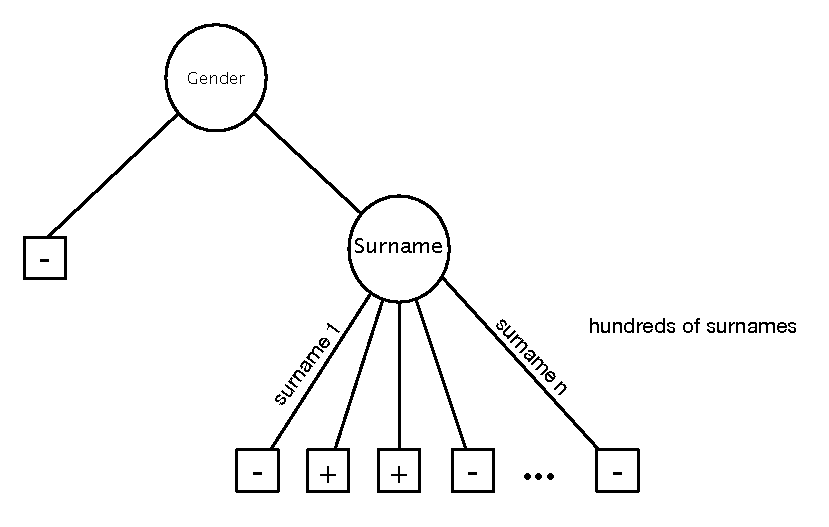
\includegraphics[width=0.8\linewidth]{fig1.pdf}
	\caption{A decision tree for the basic features}
	\label{fig:tree_base}
\end{figure}

The above example illustrates that without additional knowledge, an induction algorithm will yield a very poor result. %Even if we attempt to use standard feature generation approaches, there is no additional information that combinations of these features would find.
However, if we assume that we have access to a relational knowledge base connecting surnames to common countries of origin, we can begin to apply knowledge-based feature generation techniques to the problem, as we can move from the domain of surnames to that of countries. 

Our goal is to separate the set of people to those at high risk and those at low risk using induction algorithms. We see that the existing feature set is insufficient to perform this task successfully. Therefore, our approach aims to construct new features for the learning task $T_1$ by recursively creating a new learning problem $T_2$. Once we have done so, we can use induction methods on $T_2$ in order to create a classifier that can be used in $T_1$. We construct $T_2$. %as follows: 

The training objects are surnames; surnames of people with the disease are labelled as positive. The features for these new objects are extracted from the knowledge base. In this case, these features are their countries of origin.
Solving the above learning problem through an induction algorithm yields a classifier on surnames that distinguishes between surnames of patients with the disease and surnames of healthy individuals. This classifier for $T_2$ can then be used as a binary feature in the original problem $T_1$ by applying it to the feature value of surname. For example, it can be used as a feature in the node of value female in Figure \ref{fig:tree_base}, yielding the tree seen in Figure \ref{fig:lvl1_tree}. 

This new feature gives us a better generalization over the baseline solution, as we now abstract the long list of surnames to a short list of countries. %We can see this as nodes in the classifier for $T_2$ are derived from multiple surnames. 
This result also allows us to capture previously unseen surnames from those countries. However, this is not a sufficient solution, as we have no way of generalizing on previously unseen countries of origin. %, and some countries may not have sufficient representation to induce an accurate classifier. %talk about not concept?


\begin{figure}[h]
	\centering
	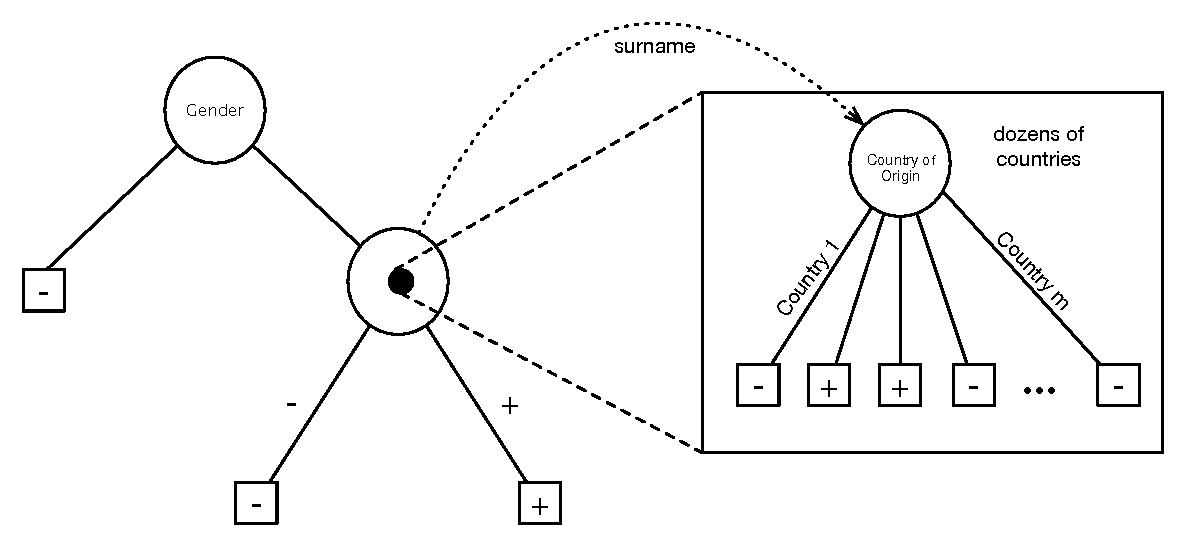
\includegraphics[width=\linewidth]{fig2.pdf}
	\caption{A constructed feature used within a decision tree}
	\label{fig:lvl1_tree}
\end{figure}

Once again, we require additional knowledge in order to capture the target concept of $T_2$. 
Therefore, we can recursively apply our method while trying to learn $T_2$ in an attempt to better locate the target concept and induce a classifier for $T_1$.
We create a new training set, the objects of which are countries of origin, with countries of surnames belonging to people with high risk are labelled as positive. The knowledge base regarding countries is then used to construct features for this new this training set, giving us a recursive learning problem $T_3$.

We can then use $T_3$ as an input to an induction algorithm. As a result of this process, we end up with a classifier for $T_3$, which tries to separate between countries of origin of people at risk and those not at risk. This classifier will do so by looking at the properties of countries, and reach the conclusion that countries with high average temperature and low precipitation are of high risk: the characteristics of desert areas.
%This classifier is then used on the country of origin feature in $T_2$, yielding a new feature for $T_2$.  This new feature can then be used when inducting a classifier for $T_2$, which, as we have mentioned earlier, is used as a feature for the original problem $T_1$.

The complete process is depicted in Figure \ref{fig:moving_to_lvl2}. %The resulting two-level recursive classifier is depicted in Figure \ref{fig:lvl2_tree}. 
This constructed feature allows us to concisely and accurately capture the target concept, as the construction process is guided by it, in a manner similar to that of deductive approaches.
%While this is a simple example, it illustrates how an unsolvable learning problem given the original features can be solved via the use of complex additional knowledge and existing induction methods.


\begin{figure*}[th]
	\centering
	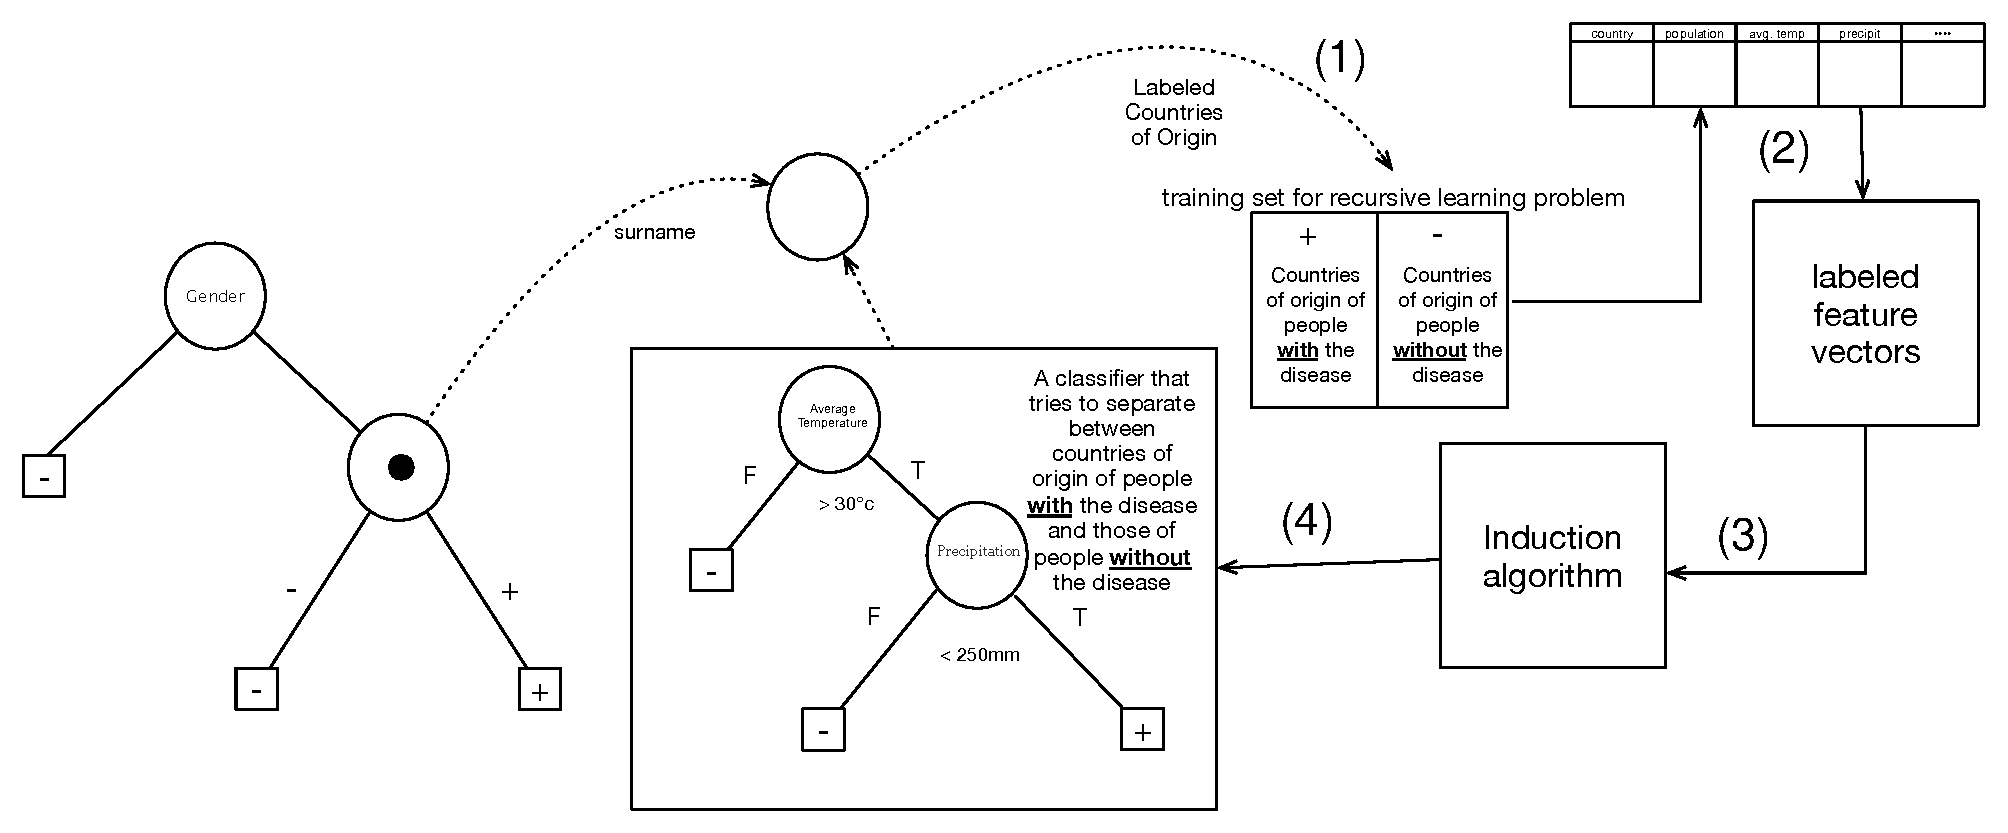
\includegraphics[width=0.9\linewidth,height=0.33\linewidth]{fig4_annotated.pdf}
	\caption{Recursive construction of a learning problem on countries of origin. $(1)$-Creating the objects for the new problem. $(2)$-Creating features using the knowledge base. $(3)$-Applying an induction algorithm. $(4)$-The resulting feature.}
	\label{fig:moving_to_lvl2}
\end{figure*}

%\begin{figure*}[th]
%	\centering
%	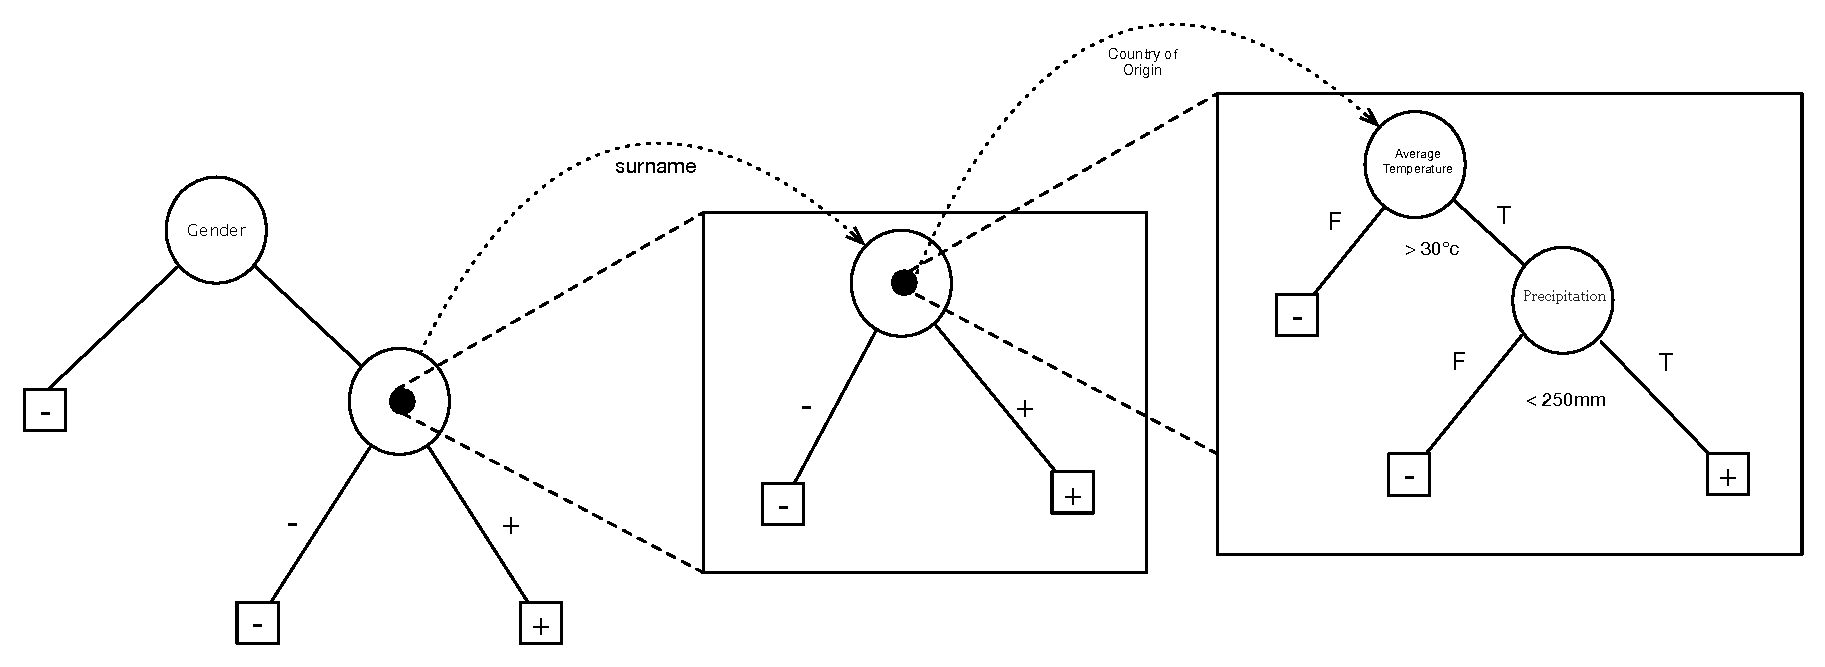
\includegraphics[width=\linewidth]{fig3.pdf}
%	\caption{A two-level constructed feature used within a decision tree}
%	\label{fig:lvl2_tree}
%\end{figure*}

%%%%%%%%%%%%%%%%%%%%%%%%%%%%%%%%%%%%%%%%%%%%%%%%%%%%%%%%%%
\section{Generating Features through Recursive Induction} \label{formal}
%%%%%%%%%%%%%%%%%%%%%%%%%%%%%%%%%%%%%%%%%%%%%%%%%%%%%%%%%%

In the following sections, we will define the feature generation problem, present a solution to that problem in the form of an unsupervised feature generation algorithm, and proceed to discuss the \emph{FEAGURE} algorithm. %TODO: why an unsupervised algorithm? 

\subsection{Problem definition}

We begin our discussion with a standard definition of an induction problem. 
Let $O$ be a set of objects. Let $Y=\{0,1\}$ be a set of labels \footnote{We assume binary labels for ease of discussion}. Let $C:O\rightarrow Y$ be a target concept. Let $S=\{(o_{1},y_{1}),\ldots,(o_{m},y_{m})\}$ be a set of labelled examples such that $o_{i}\in O, y_{i}\in Y, C(o_i)=y_i$. 
Let $F=\{f_{1},\ldots,f_{n}\}$ be a \emph{feature map}, a set of \emph{feature functions} $f_{i}:O\rightarrow I_{i}$.  This definition implies a training set represented by feature vectors: $S_F=\{ (\langle f_1(o_i),\ldots,f_n(o_i)\rangle, y_i) | (o_i,y_i) \in S\}$. A learning algorithm $L$ takes $S_F$ as inputs, and outputs a classifier $h_{S_F}:O\rightarrow Y$.
\begin{defn}
	Let $L(S,F)=h_{S_F}$ be the classifier given as an output by $L$ given $\langle S,F\rangle$. Assuming $S\sim\ D$, the generalization error of a learning algorithm $L$ is the probability $Pr(h_{S_F}(x)\neq y)$, where $(x,y)\sim\ D$.
\end{defn}

\begin{defn}
	A \emph{feature generation algorithm} $A$ is an algorithm that given $\langle S,F\rangle$, creates a new feature map $F'=\{f'_{1},\ldots,f'_{l}\}, f'_{k}:O\rightarrow I_k$.
\end{defn}

In order to evaluate the output of a feature generation algorithm $A$, we must define its utility. Given $\langle S,F \rangle$, $A$ generates a feature set $F'_A$.
Given $S\sim\ D$, a feature set $F$, a generated feature set $F'_A$ and a learning algorithm $L$, the utility of $A$ is $U(A(S,F))=Pr(h_{S_F}(x)\neq y)-Pr(h_{S_{F'_A}}(x)\neq y)$, where $(x,y)\sim\ D$.

Thus, if the classifier induced by $L$ given  $\langle S,F \rangle$ yields a low generalization error, the utility will be low, and in order for the utility of $A$ to be positive, the generated feature set $F'_A$ must yield a lower generalization error compared to $F$.

In this work, we assume that in addition to $S_F$, $A$ also has access to a set of binary\footnote{If our relations are not binary, we can use projection to create multiple binary relations instead} relations ${\cal R}=\{R_{1},\ldots,R_{t}\}, R_j:D_j\times D_{j'}$ representing our knowledge base. 
\begin{defn}
	A \emph{knowledge based feature generation algorithm} $A$ is an algorithm that given $\langle S,F,{\cal R} \rangle$, creates a new feature map $F_{{\cal R}}=\{f'_{1},\ldots,f'_{l}\}, f'_{k}:O\rightarrow I_k$.
\end{defn}

%When using a feature generation algorithm based on a set of relations ${\cal R}$, we would like to achieve a higher utility than that achieved without the use of ${\cal R}$. We assume that some feature values are also relation keys, allowing us to apply these relations to our learning problem. More formally, we assume 
% $\bigcup_{f_i} I_i \cap \bigcup_{R_j} D_j \neq \emptyset$. 

\subsection{An approach to knowledge-based feature generation} \label{shallow_section}

To begin with, we shall treat the example set $S$ as unlabelled, and define an unsupervised knowledge based feature generation algorithm based on ${\cal R}$ named \emph{Expander-FG}. %, as it uses the relations to expand existing features. Using \emph{Expander-FG}, we can highlight several important concepts of our approach.

%Let us first consider the simplest case, where any given relation $R_j$ is a function $R_j:D_j\rightarrow D_{j'}$. 
%If a relation $R_j$ is a function, then for any given $f_i$ such that 
%$Image(f_i) \subseteq D_j$, we can generate a new feature function $f_{i,j}:O\rightarrow D_{j'}$ by composing $R_j$ onto $f_i$, yielding our new feature function  $f_{i,j}(x)=R_j\circ f_i=R_j(f_i(x))$.
%Thus we can define the feature generation algorithm \emph{Expander-FG} using a closed formula: $\{f_{i,j}=R_j\circ f_i|Image(f_i) \subseteq D_j\}$.
For any relation $R_j$, if $Image(f_i) \cap D_j \neq\emptyset$, we can generate a new feature function $f_{i,j}:O\rightarrow D_{j'}\cup\{\perp\}$ ($\perp$ is the undefined symbol) by composing $R_j$ onto $f_i$ when applicable, yielding our new feature function  $f_{i,j}(x)=\tilde{R_j}\circ f_i$, where $\tilde{R}_j(x)=\begin{cases} R_j(x) &\mbox{if } x\in D_j\\ 
\perp & \mbox{otherwise } \end{cases}$.

%Another case that must be discussed is the case where some values of $f_i$ cannot be expanded as above, meaning $Image(f_i) \not\subset D_j$ but $Image(f_i) \cap D_j \neq\emptyset$. We can resolve this in a manner similar to missing features in induction problem, by treating $R_j$ as a partial function from $Image(f_i)$ to $D_{j'}$. In order to complete this partial function, we first mark \emph{undefined} as $\perp$. We can turn $R_j$ into a full function with regards to $Image(f_i)$ as follows: $\tilde{R}_j(x)=\begin{cases} R_j(x) &\mbox{if } x\in D_j\\ 
%\perp & \mbox{otherwise } \end{cases}$.
%The result is a full function $\tilde{R}_j:Image(f_i)\cup D_j\rightarrow D_{j'}\cup\{\perp\}$. We also note that the same process can be applied to cases where $R_j$ has missing values\footnote{This is usually the case in human curated knowledge bases.}, meaning it is a partial function with regards to $D_j$. 

In the general case, composing $R_j$ onto $F_i$ yields a set of values, meaning $f_{i,j}(x)=\{v\in D_{j'}|(f_i(x),v)\in R_j\}$. 
%This set can be used as a set-based feature, but since the number of possible sets is exponentially larger than the number of values, it is usually better to utilize an aggregation function on the set of values instead. 
We use on aggregation function on this set.
%An aggregation function is a function that given a multi-set as input, outputs a single value. There are many types of aggregators, such as numerical aggregators (i.e. sum), categorical aggregators (i.e. most common member) and binary aggregation functions (i.e. exists).
We will make use of two aggregation function families: Majority and Any.
For each value $v\in D_{j'}$, we can define Majority as follows:
 
$Majority^v(X)=\begin{cases} 1 &\mbox{if } majority(X)=v
\\ 
0 & \mbox{otherwise } \end{cases}$

Using these functions, we can turn one generated feature $f_{i,j}$ into a set of binary features. %by applying the set of aggregation functions. 
For example:  $F_{i,j}^{Majority}=\{Majority^v(f_{i,j})|v\in D_{j'}\}$

%Now that we have considered the possible behaviours of a given relation $R_j$, we can proceed to define the \emph{Expander-FG} feature generation algorithm. Given a feature $f_i$, \emph{Expander-FG} will go over the relations within the knowledge base and attempt to create features $f_{i,j}:O\rightarrow D_{j'}\cup\{\perp\}$ through the discussed techniques. \emph{Expander-FG} then gathers all generated features and outputs them. The pseudo-code is given below.

\begin{algorithm}[H]
	\caption{\emph{Expander-FG}: Knowledge-based feature generation}
	\label{code-compete}
	\small
	$\sigma$ - An aggregation function family
	\begin{algorithmic}
		\Function{GenerateFeatures}{$S$,$F$, ${\cal R}$}
		\State $generated=\emptyset$
		\For {$f_i \in F$}
		\For {$R_j \in {\cal R}$}
		\If {$Image(f_i)\cap D_{j}\ne\emptyset$}
		\If {$R_j$ is a function}
		%\If {$Image(f_i)\subseteq D_{j}$}
		%\State add $\{f_{i,j}=R_j\circ f_i\}$ to $generated$
		\If {$Image(f_i)\cap D_{j}\neq\emptyset$}
		\State add $\{f_{i,j}=\tilde{R}_j\circ f_i\}$ to $generated$
		\EndIf
		\Else \Comment $R_j$ is a relation $R_j:D_j\times D_{j'}$
		\State add $F^\sigma_{i,j}=\{\sigma^v(f_{i,j})|v\in D_{j'}\}$ to $generated$
		\EndIf
		\EndIf
		\EndFor
		\EndFor
		\State \Return $generated$ 
		\EndFunction
		
	\end{algorithmic}
\end{algorithm}

\subsection{FEAGURE-FEAture Generation Using REcursive induction}
\label{algorithm_section}

We have seen how \emph{Expander-FG} can be used as a feature generation algorithm.
Should we try to apply it more than once, we would get more complex features. We would also, however, experience an exponential increase in the number of generated features.
%The approach shown in \emph{Expander-FG} has one major issue, which is that the algorithm only uses the relations for a single hop, from feature values to the relation domain.
%\begin{itemize}
%	\item The size of the generated feature set is much larger than the original f%eature set (especially when aggregation is used).
%	\item The algorithm only uses the relations for a single hop, from feature values to the relation domain.
%\end{itemize}
%We could potentially resolve this issue by applying \emph{Expander-FG} to the generated features, giving us additional hops and thus more complex features. The downside of this expansion is that it causes an exponential increase in the number of generated features.

To that end, we propose an alternative knowledge-based feature generation algorithm. Given the input $\langle S,F,{\cal R} \rangle$, for each feature $f_i\in F, f_i:O\rightarrow I_i$, our algorithm will create a recursive problem whose objects are the values of $f_i$, where values associated with positive examples in $S$ are labelled positive. %, and those associated with negative examples labelled negative. 
Features for this generated problem will be created using the relations in ${\cal R}$. Once this new learning problem $\langle S'_i,F'_i\rangle$ is defined, an induction algorithm is used to create a classifier $h_i:I_i\rightarrow Y$. Finally, our algorithm outputs a single generated feature for $f_i$, $f'_i(x)=h_i\circ f_i=h_i(f_i(x)), f'_i:O\rightarrow Y$.
We name this algorithm \emph{FEAGURE} (FEAture Generation Using REcursive induction).

We note that during the construction of our recursive learning problem, we can apply a feature generation algorithm on $\langle S'_i,F'_i,{\cal R} \rangle$. In particular, we can apply \emph{FEAGURE} to the constructed learning problem.%, hence the word ``recursive" in its name.

%\subsubsection{Creating Learning Problems using Relations}  

Given a feature $f_{i}$, we would like to create a recursive learning problem $\langle S'_i,F'_i \rangle$. %In this section, we will discuss how we do so.
For each feature $f_{i}$, we first define $v_i(S) = \{v | (o,y) \in S, f_{i}(o)=v\}$ the set of feature values for $f_i$ in the example set $S$. %In the intro example, for instance, $v_i(S)$ will be the set of all last names of patients that appeared in the training set.
We use $v_i(S)$ as our set of objects.

In order to define a learning problem, we must label this new set of objects $v_i(S)$. If there is only a single example in the training set $S$ such that $f_i(o)=v$, then the label of $v$ will be the label of $o$. Otherwise, we take the majority label - the most common label of objects in $o\in S$ such that $f_i(o)=v$. More formally, $label(v)=majority(\{y|(o,y)\in S, f_i(o)=v\})$.

%We now formulate a new learning problem with the constructed training set
%$S'_i = \{ (v, label(v)) | v \in v_i(S) \}$.
To fully define our learning problem, we must specify a feature map over $v_i(S)\subseteq Image(f_i)$. In a similar manner to \emph{Expander-FG}, we use the relations in ${\cal R}$ on the elements in the new training set $S'_i$.
Given $R_j$, assuming it is relevant to the problem domain, meaning $v_i(S)\cap D_j\neq\emptyset$, we can utilize it as a feature $R_j(v)$. 
The result of this process is a feature map for $S'_i$ that includes all such relations,, denoted as $F_{\cal R}$. %TODO: mby this is a bit laconic? needs more?

We now have a complete induction problem $\langle S'_i,F_{\cal R} \rangle$ for which we can train a classifier, giving us $h_i:I_i\rightarrow Y$. We can then use this $h_i$ on objects in $S$ as discussed above, giving us a new feature $f'_{i}(x)=h_{i}(f_{i}(x)), f'_{i}:O\rightarrow Y$. 

%We note that once we have an induction problem over $I_i$, we can apply our approach recursively on $S'_i$ in order to create additional features. We can see an example of this in section \ref{motivation}, wherein we construct a second-level problem on countries of origin to correctly identify the appropriate conditions that signify high risk countries.

Since it is possible for the value of a feature $f_i$ to be a set, we must address this case as well. For construction of a recursive problem, each element takes the label of the example. When applying the newly constructed classifier to the values of $f_i$, we use the majority function to decide on the value.%, as demonstrated in Figure \ref{figure5}.

%In some cases, the feature function used may map an example to a set of values rather than a single one% (for example, when we apply our approach recursively).
%In such cases, we label all feature values for a given training example using the label of that example.
%An additional concern is that when the newly constructed classifier $h_i$ is applied to the values of $f_i$, the result is a set of labels. To illustrate this, we look at the classifier shown in Figure \ref{figure5}. We see that this classifier can be applied to the multiple values of the feature, giving us a set of labels. We then apply the majority function to yield a single value for this training example.

%\begin{figure}[t]
%	\centering
%	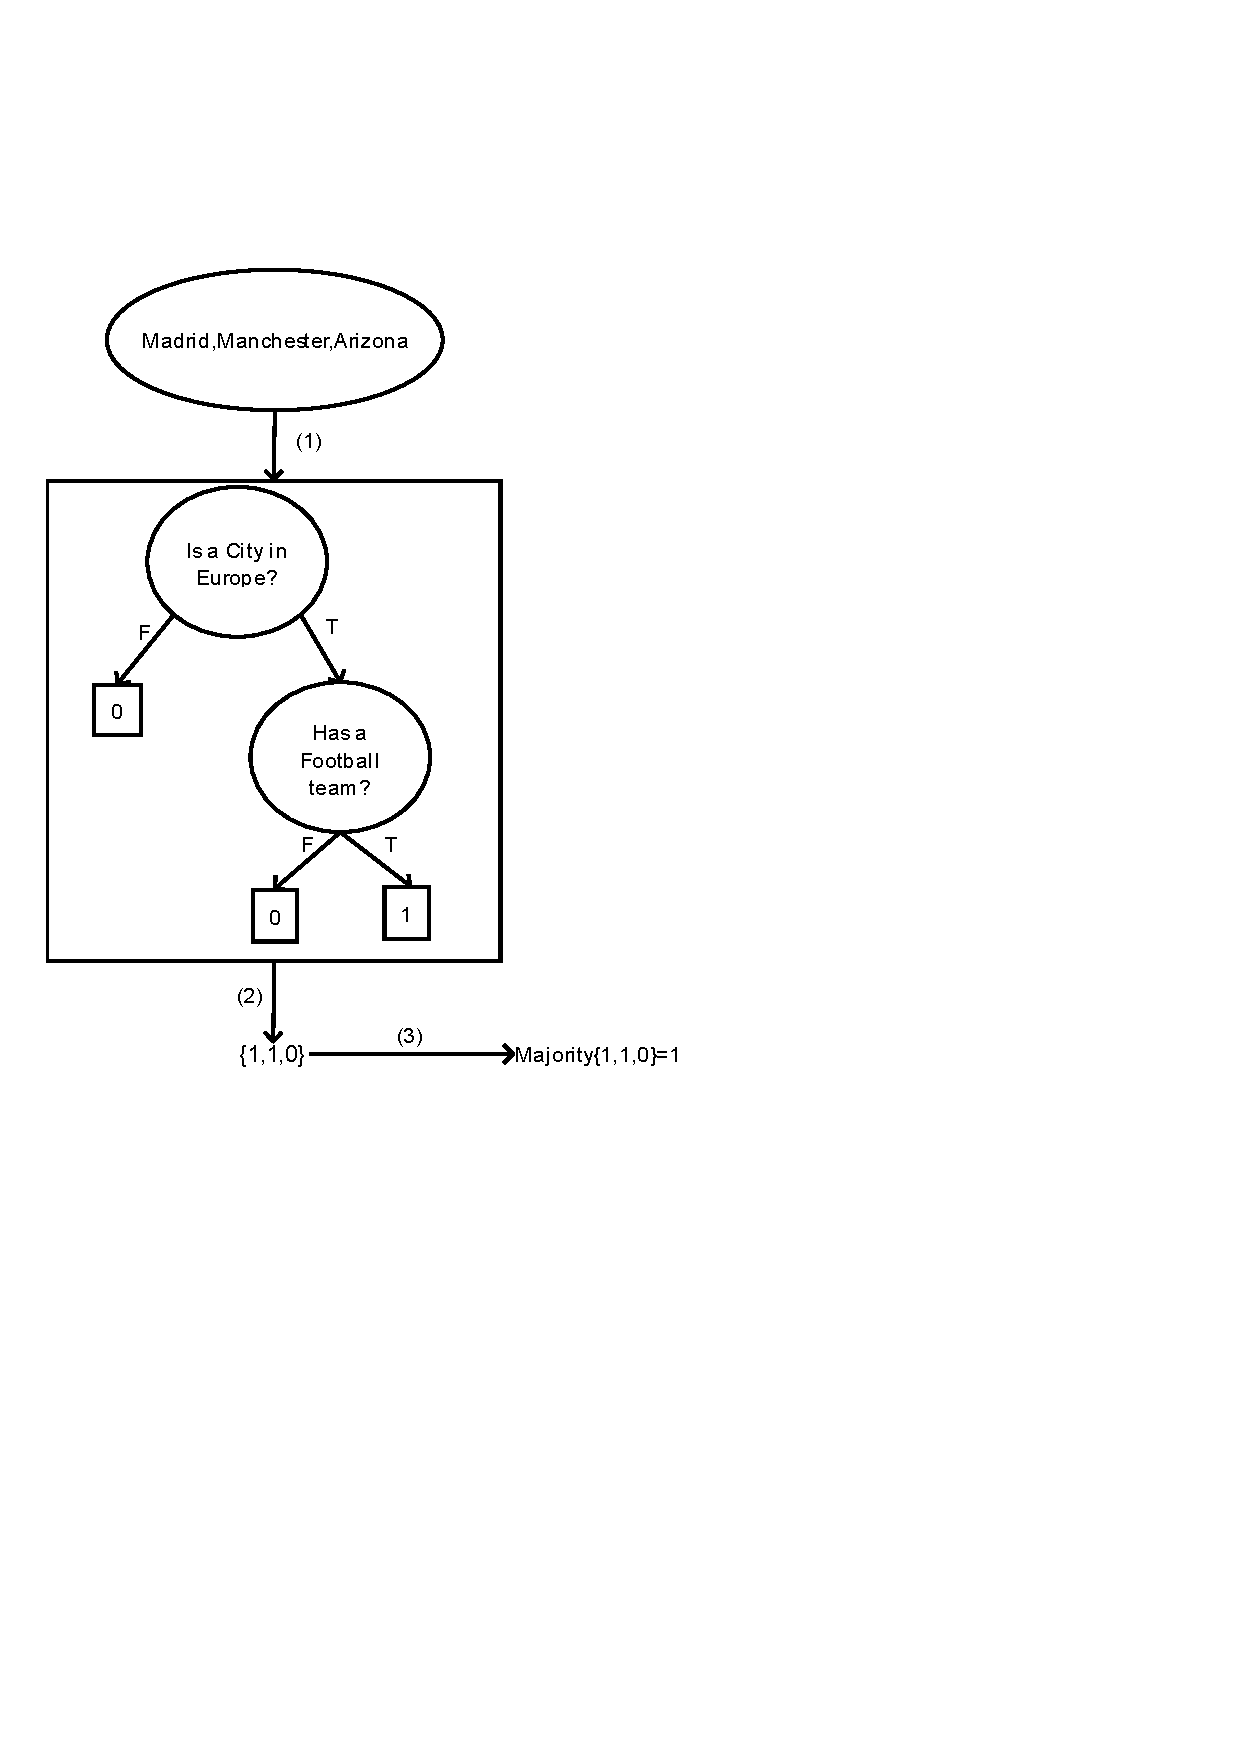
\includegraphics[height=0.6 \linewidth]{fig6.pdf}
%	\caption{Using a constructed classifier on a set of values: $(1)$-Feature values are used to construct a learning problem. $(2)$-The classifier is then applied to each value. $(3)$-The majority function is used to determine the output for the training example.}
%	\label{figure5}
%\end{figure}

%\subsubsection{Feature Selection} %TODO: stands out too much! small? part of tree? move to 4?

%In many feature generation approaches, feature selection methods play a key part in filtering out poor features. In FEAGURE, we can use feature selection both as a filtering mechanism, as well as a search parameter.
%As a filtering technique, the features generated by FEAGURE are compared to the already existing feature map $F$. There is a multitude of feature selection techniques that can be applied for this task, but we shall cover three filtering criteria.
%\begin{enumerate}
%	\item Maximal Information Gain (IG)- The information gain metric \cite{quinlan1986} compares how well a single feature reduces the amount of information entropy within a given labelled set should we split by it. In essence, it measures how well each feature separates the set based on its labels. Taking the maximal information gain as a metric, we measure whether the constructed feature gives a better separation compared to all existing features in $F$.
%	\item Average Information Gain- Just as we can compare our feature to the maximal IG of the feature map, we can compare it to the mean IG for features in $F$.
%	\item Sufficient Diversity- IG based approaches measure the separation of the training set. In many feature generation tasks, however, the more correct approach is to generate features which differ from existing features. To do so, we could require that the correlation of the generated feature with features in $F$ be below a certain threshold.
%\end{enumerate}
%Beyond their use for filtering, criteria that measure the performance of features such as the ones above can be used as a deciding factor in whether or not a constructed learning problem should apply FEAGURE recursively. The idea here is that should the generated feature be close to the threshold, we may wish to continue expanding it in hopes of giving that feature the necessary boost in terms of the specific criteria.

\begin{algorithm}[H]
	\caption{FEAGURE-FEAture Generation Using REcursive induction}
	\label{code-creating-prob}
	\small
	%insert param stuff
	\begin{algorithmic}
		\Function{GenerateFeatures}{$F$, $S$, ${\cal R}$}
		\For {$f_i\in F$}
		\State $S'_i,F_{\cal R}$= \Call{CreateNewProblem}{$f_i$,$S$,${\cal R}$} %\Comment{We can apply our algorithm recursively here}
		\State $h_i$= \Call{InductionAlgorithm}{$S'_i,F_{\cal R}$} 
		%\If {\Call{Compare}{$h_i,F$}} \Comment Compare $h_i$ to $F$
		\State add $h_i$ to generated features
		%\EndIf
		\EndFor
		\State \Return generated features
		\EndFunction
		\State 
		\Function{CreateNewProblem}{$f_{i}$, $S$, ${\cal R}$}
		\State $v_i(S) = \{v | (o,y) \in S, f_{i}(o)=v\}$
		\State $S'_i = \{ (v, majority-label(v)) | v \in v_i(S) \}$ 
		%\Comment $label(v)$ is the majority function.
		
		\State $F_{\cal R}=\{f_{j}=R_j(v)| R_j\in{\cal R}\}$
		\If {Should apply recursively}
		\State $F_{\cal R}=F_{\cal R}\cup$\Call{GenerateFeatures}{$F_{\cal R}, S'_i,  {\cal R}$}
		\EndIf
		\State \Return $S'_i, F_{\cal R}$ 
		\EndFunction
		
	\end{algorithmic}
\end{algorithm}

%We note that this feature generation approach creates features that can be used alongside any induction algorithm. Additionally, any induction algorithm can be used to learn $h_i$. Due to this generality, the extensive knowledge and literature available for induction methods applies in full. Furthermore, the recursive nature of \emph{FEAGURE} allows for a structured search of the knowledge base, with each new recursive problem modelling a projection of the problem space to the new domain, allowing for a process similar to deductive learning. For example, in the motivating example, we began by learning a problem regarding patients, which we projected to a new domain of surnames. We then re-contextualized that problem to the domain of countries, for which we located a good solution. We then used this solution to resolve the original learning task concisely and accurately.
%TODO: mby we want to keep some of this...

%TODO: missing info on when to stop...

%\subsection{Finding Locally Improving Features} \label{tree_usage}

%In many cases, it is easier to locate powerful features within a localized subset of data which shares common attributes rather than trying to locate the same features in a more global context. In the motivating example, for instance, male patients are irrelevant to the target concept, and thus serve as noise when used for feature generation.
%There is a multitude of approaches to creating such local features. We shall consider a few of these approaches:
%\begin{itemize}
%	\item Sub-Sampling: By sampling a subset of training examples, we can hope to create a good local context for feature generation. An issue with this approach is that there is a huge number of possible subsets, and thus going over all of them is not computationally feasible. 
%	\item Clustering: This approach attempts to make use of the feature set to create clusters of similar examples. In some cases, this would indeed yield good local contexts, but this approach is potentially problematic for our algorithm, as it is very likely that similar examples will have the same label, thus creating highly unbalanced learning problems, which would be more difficult to utilize effectively.
%	\item Divide \& Conquer: This approach seeks to iteratively create increasingly smaller subsets of the original problem by dividing the problem according to the values of a feature. Most often, the IG metric is used to determine the feature used to split the examples.
%\end{itemize}

%One approach to creating such local contexts is the Divide \& Conquer approach. This approach seeks to iteratively create increasingly smaller subsets of the original problem by dividing the problem according to the values of a feature. One way to do so is to make use of the information gain \citep{quinlan1986} metric to determine the feature used to split the examples. The Divide \& Conquer approach has numerous advantages we can make use of, namely:
%\begin{enumerate}
%	\item Orthogonality: Because all examples with the same value for a given feature are grouped together, any further splits must make use of different features. %Due to this and the fact that the features selected in each step have high IG, it is usually the case that features chosen later in the process will be mostly orthogonal to previously chosen features. %This results in a larger variety of features overall. In our approach in particular, the elimination of a feature prunes the search tree and forces later splits to rely on different features and thus different domains.
	%\item Interpertability: Looking at the features used at each splitting point gives us an intuitive understanding of the resulting subsets. %Because of this, we can more easily understand why certain features were picked over others, which domains are no longer relevant, and so on.
	%\item Iterative construction: The divide \& conquer approach allows for an iterative search process.%, which we can then easily interrupt if a sufficient number of features were generated, or when the remaining training set is no longer sufficiently representative for drawing meaningful conclusions.
	%\item Guided by labelling: This approach explicitly uses the labels of the training set to create meaningfully different groups. %As a result of this, we can expect that as we go further down, the need for good, distinguishing features will rise, and we can locate stronger features.
%\end{enumerate}

%We define a new feature generation algorithm based on the divide \& conquer approach. To begin with, we take the training set and generate features for it using \emph{FEAGURE}. We keep the generated feature, and the feature with the highest information gain is used to split the training set into groups. We then apply this process recursively for each group until a group is either too small or has consistent labels. Once done, we return the combined set of features from all groups. We name this new algorithm \emph{Deep-FEAGURE}.

%Due to the above advantages, we have a strong incentive to utilize the divide \& conquer approach when attempting to create additional features using \emph{FEAGURE}. This new feature generation algorithm, which we shall name \emph{Deep-FEAGURE}, begins by taking the entire training set and applying \emph{FEAGURE} to it. Once features have been generated, any generated features that have performed well are kept, and the feature with the highest information gain (potentially the one generated by \emph{FEAGURE}) is used to split the training set into groups according to its values.
%We then repeat this process for each of these new, smaller training sets, until we either receive a consistent training set, meaning all examples have the same label, or the size of the training set becomes so small that it is wholly unrepresentative of the complete problem.
%Once we have finished this process, the generated features are returned as the output of \emph{Deep-FEAGURE}.
%TODO: performed well is undefined...

%A major potential issue that must be considered in any induction approach, and is especially problematic for divide \& conquer approaches, is that of over-fitting, meaning that the result is too adjusted to seen data, and cannot generalize to previously unseen data. In the extreme case, an induction method may yield a classifier that simply memorizes the known data, and is thus incapable of generalization.
%TODO: mby we want to keep this?
%To combat this issue, we consider several steps:
%\begin{itemize}
%	\item Limiting the minimal size of the training set allows us to control for unrepresentative subsets, which is a major factor in over-fitting.
%	\item Feature selection approaches can be used on the output of \emph{FEAGURE} in order to limit the potential for over-fitting. It is important to mention, however, that a very strict feature selection criterion may have an opposite effect, as any feature that pass it must be very well fitted to the training data.
%	\item Limiting the depth of search by refusing to further split beyond a certain depth is another way to prevent unrepresentative subsets. Of particular notice, the number of relations in our knowledge base gives us a natural depth limit due to the orthogonal nature of this approach. Essentially, once a certain relation has been used, it is unlikely that another feature down the tree will make use of it again, as we have already split the training set according to values of that domain. 
%	\item Well-known induction approaches often acknowledge the issue of over-fitting, and offer multiple techniques to minimize it. Should we use search trees, for example, flattening can be used to create a set of weaker features, which is less likely to over-fit than a single complex decision tree.
%\end{itemize}

%\begin{algorithm}[H]
%	\caption{Deep FEAGURE- Divide \& Conquer Feature Generation}
%	\label{code-tree-thing}
%	\small
%	minSize- minimal size of a node.
	
%	SplitByBestFeature- splits a training set according to a feature.
	
%	\begin{algorithmic}
%		\Function{GenerateFeaturesInANode}{$S$, $F$, ${\cal R}$}
%		\If {$|S|<$minSize} \Comment We can also apply other steps.
%		\State
%		\Return 
%		\EndIf
%		\State newFeatures=\Call{FEAGURE}{$S$, $F$, ${\cal R}$}
%		\State \Return \Call{SplitByBestFeature}{$S$, $F\cup$ newFeatures}, newFeatures
%		\EndFunction
		
		
%		\State 
%		\Function{GenerateFeatures}{$S$, $F$, ${\cal R}$}
%		\State currentFeatures= $\emptyset$
%		\State sons, $F_{new}$=\Call{GenerateFeaturesInANode}{$S$, $F$, ${\cal R}$}
%		\State currentFeatures= currentFeatures$\cup F_{new}$
%		\For {son in sons}
%		\State newFeatures=\Call{GenerateFeatures}{son.$S$,$F$,${\cal R}$}
%		\State currentFeatures= currentFeatures$\cup$newFeatures
%		\EndFor
%		\State \Return currentFeatures
%		\EndFunction
%	\end{algorithmic}
%\end{algorithm}


%%%%%%%%%%%%%%%%%%%%%%%%%%%%%%%%%%%%%%%%%%%%%%%%%%%%%%%%%%
\section{Empirical Evaluation}
%%%%%%%%%%%%%%%%%%%%%%%%%%%%%%%%%%%%%%%%%%%%%%%%%%%%%%%%%%
In this section, we discuss our experimental methodology, detail the algorithms, datasets and knowledge bases we utilize and display our main results.

%%%%%%%%%%%%%%%%%%%%%%%%%%%%%%%%%%%%%%%%%%%%%%%%%%%%%%%%%%
\subsection{Application of FEAGURE for Text Categorization} \label{text-feagure}
%%%%%%%%%%%%%%%%%%%%%%%%%%%%%%%%%%%%%%%%%%%%%%%%%%%%%%%%%%

One interesting problem domain for FEAGURE is that of \emph{Text Categorization}.
%The text categorization problem is defined by a set of texts $O$ labelled by a set of categories $Y$ \footnote{We can assume $Y=\{0,1\}$ for ease of analysis}
%such that we create $S=\{(o_i,y_i)|o_i\in O, y_i\in Y\}$. Given $S$, The learning problem is to find a hypothesis $h:O\rightarrow Y$ which minimizes generalization error over all possible texts of the given categories. To measure this error, a testing set is used as an approximation.
The traditional approach to solving this problem is based on the bag-of-words \citep{Wu:1981:CST:1013228.511759} approach, which uses the frequencies of word appearances within the text as features. 

Another way to describe this approach is that it creates a single feature, the titular bag-of-words, whose value is the set of all unique words in the text.
%As we are well aware, however, not all words have semantic meaning. This observation makes usage of knowledge-based approaches non-trivial, as most knowledge bases rely on semantically meaningful entities rather than raw words.
%To resolve this issue, we can make use of techniques such as Named Entity Recognition (NER), Wikification \cite{bunescu2006using} and Entity Linking \cite{rao2013entity}. These methods as well as similar techniques allow us to link words in the text with semantically meaningful entities. 
Using entity linking techniques \citep{bunescu2006using,rao2013entity}, we can move to a \emph{bag-of-entities} representation, a model of the semantically meaningful entities within the text.

%As discussed, we have seen the recent rise of Semantic Linked Data as a powerful knowledge base for text-based entities, with large databases such as Google Knowledge Graph \cite{pelikanova2014google}, Wikidata \cite{vrandevcic2014wikidata} and YAGO2 \cite{hoffart2013yago2} becoming common. 
%These knowledge bases represent semantic knowledge through the use of relations, mostly represented by triplets of various schema such as RDF, or in structures such as OWL and XML. These structures conform to relationships between entities such as "born in" (hyponyms), as well as type information (hypernyms).
%Naturally, we would like to make use of such semantic data to improve upon the bag-of-words and bag-of-entities approaches, with the implicit assumption that additional semantic knowledge will allow us to better approximate the relationship between a text and its given category.

Since entities belong to different domains (such as people and locations), different relations apply to such entities. In order to better create relevant features, we consider only entities in the same domain, using the relations within the knowledge base as indicators of such domains. For instance, given the whole bag-of-entities, we might look at entities that are keys in the ``died in" relation, thus giving us only entities that correspond to deceased people.

%A major topic to consider when trying to apply \emph{FEAGURE} to this domain is the fact that the bag-of-entities approach inherently creates features with many values. %Because of this, special care must be taken to both the construction of recursive problems (a single example may have multiple values and thus contribute to many examples in the recursive problem) and the application of the resulting classifier on the document (aggregation over the values may be required).
%Naturally, many entities within a given document will not apply to a given relation as the domains differ, and thus yield a value of $\perp$. To combat this, we only yield a feature value of $\perp$ for a given document if that document contains no entities that are relevant to the constructed classifier.
%TODO

%\subsection{Algorithms}

%In order to test the effectiveness of \emph{FEAGURE}, we compared three feature generation algorithms:
%\begin{enumerate}
%	\item \emph{Expander-FG}: This unsupervised algorithm, defined in section \ref{shallow_section} allows us to see the effects of the knowledge base on accuracy in general. %Through this algorithm, we can better measure the effectiveness of \emph{FEAGURE}.
%	\item \emph{FEAGURE}: We applied \emph{FEAGURE} to the learning problem, and constructed recursive learning problems. Each such new problem was then solved and used as a feature.
%	\item \emph{FEAGURE} 2-level: This algorithm is the 2-level application of \emph{FEAGURE}, as demonstrated in section \ref{motivation}. During the activation of \emph{FEAGURE}, we applied the algorithm recursively on each generated learning problem.%, allowing us to locate deeper relationships within the dataset.
%\end{enumerate}

\subsection{Methodology}

We have evaluated our algorithm in the domain of text categorization problems.
%A%s we have discussed in section \ref{formal}, in order to evaluate a feature generation algorithm, we must first define an induction problem in order to measure generalization error and utility. Once we have defined the problem, we activate the feature generation algorithm on the training set in order to generate new features. We proceed to test the generated feature set by learning a classifier on the expanded training set and measuring its accuracy against a testing set %\footnote{This testing set is treated as a sample of the object space $O$}
%, compared to the baseline approach without the use of feature generation.
We measured the utility of our feature generation algorithm as described in section \ref{formal}.

 We made use of three well-known learning algorithms for this task: SVM \citep{cortes1995support}, K-NN \citep{fix1951discriminatory} and CART \citep{breiman1984classification}%\footnote{For SVM we used a linear kernel and a regularization parameter $C=10$; for K-NN we used $K=3$; for CART we used a minimal leaf size proportional to training set size}.
%The use of multiple induction algorithms allowed us to reduce the impact of the specific induction approach in evaluating the performance of the generated features.


%\subsubsection{Datasets and Knowledge Bases}

%In order to best evaluate our approach, we wished to test it on a wide array of text classification datasets. To that end, we focused on the TechTC-100 \citep{gabrilovich2004text} dataset collection.

\textbf{TechTC-100} \citep{gabrilovich2004text} is a collection of 100 different binary text categorization problems of varying difficulty, extracted from the Open Dictionary project.
We evaluated our approach by measuring accuracy based on the training and testing sets defined in the original paper. 

As our knowledge base for this task, we used YAGO2 \citep{hoffart2013yago2}.
YAGO2 (Yet Another Great Ontology) is a large general knowledge base extracted automatically from Wikipedia, WordNet and GeoNames.
YAGO2 contains over 10 million entities and 124 million facts, mostly dealing in individuals, countries and events.
%In order to fully make use of this knowledge base, we performed some processing on it. Specifically, we omitted relations with literal data such as dates or geographic coordinates, and created inverse relations of all relations except ones that map very few values to very many \footnote{For example, the inverse of the ``has gender" relation  maps ``male" and ``female" to all to all existing people within the YAGO2 database.}.

For entity extraction, we used AIDA \citep{hoffart2011robust}, a framework for entity detection and disambiguation. %AIDA uses the Stanford NER tagger \cite{finkel2005incorporatingfull} to locate entity candidates, and attempts to link them to existing entities within the YAGO2 knowledge base.

%The TechTC-100 dataset collection served as a powerful benchmark, as it shows results for multiple problems at once, giving a broad view for many problems with varying difficulties. This aspect allowed us to better understand and analyse our approach in a variety of situations.
%TODO

%We also wanted to explore the results of our approach with regards to a more domain-specific problem.
%To that end, we constructed a dataset based on OHSUMED \citep{hersh1994ohsumed}.

\textbf{OHSUMED} \citep{hersh1994ohsumed} is a large dataset of medical abstracts from the MeSH categories of the year 1991. 
We constructed our own dataset based on the work of \citep{joachims1998text}.
First, we took the first 20,000 documents, similarly to \cite{joachims1998text}.
Then, we limited the texts further to medical documents that contain only a title. %On each document, we used stopword elimination, a simple stemming scheme %(due to the medical nature of the texts, there was no need for complex stemming) in order to remove unnecessary noise. Once the documents have been cleaned of stopwords and stemmed,
Due to the relatively sparse size of most MeSH categories, we only used the two categories with the most documents, C1 and C20. %``Bacterial Infections and Mycoses" and ``Immunologic Diseases"\footnote{C1 and C20, respectively}, yielding a binary learning problem.
The result is a dataset of 850 documents of each category, for a total of 1700 documents.
Ten-fold cross validation was used in order to evaluate the accuracy of algorithms on the dataset and measure statistical significance.

%As the YAGO2 knowledge base does not contain medical facts, we sought to use a more appropriate knowledge base for our task. To that end, we opted to use \textbf{Freebase}.
For our knowledge base, we took the Freebase data dump used by \cite{bast2014easy}. Freebase has been described as ``a massive, collaboratively edited database of cross-linked data". Freebase is constructed as a combination of data harvested from databases such as Wikipedia and data contributed by users. The result is a massive, extensive knowledge base containing 1.9 billion facts. 

We used Wikipedia Miner \citep{milne2013open} for entity extraction. 
%We used the same freebase data dump used by \cite{bast2014easy}, taking only entities relevant to our domain. 
%This smaller dump of the Freebase knowledge base contains approximately 49 million entities and 242 million facts spanning multiple domains. Data regarding the medical domain is far more sparse, containing roughly a hundred thousand facts in total.

%Due to it's inclusion of domain specific knowledge, Freebase is more suitable for problems specializing in a specific subject, such as the OHSUMED dataset. 
%This dataset served as a test case for a more specialized learning problem, where domain-specific knowledge is required.
%TODO

%In general, we do not expect a single knowledge base to effectively apply to any and all problem domains, but rather that each problem domain make use of a more tailored, domain-appropriate knowledge base. By doing so, we can hope to better solve these problems.
%TODO

%\subsubsection{Experiment Parameters}

%We tested the following parameters: 
%\begin{enumerate}
%	\item Recursion level: We ran our feature generation algorithm for both a depth of one, creating a recursive learning problem for the original problem, and a depth of two, creating recursive learning problems within generated problems. This parameter allowed us to test the effect of both first and second order application of our feature generation approach.
	
	%\item \emph{FEAGURE} internal induction algorithm: In section \ref{algorithm_section}, we define \emph{FEAGURE} without specifying the internal induction algorithm used to generate features within the new learning problem. We ran most of our experiments using a decision tree induction algorithm for that purpose, flattening the result to yield additional features. We also experimented with the use of other induction algorithms, namely SVM and K-NN.
	
%\end{enumerate}


%%%%%%%%%%%%%%%%%%%%%%%%%%%%%%%%%%%
\subsection{Main Results}
%%%%%%%%%%%%%%%%%%%%%%%%%%%%%%%%%%%

Table \ref{table:acc} shows average accuracies across all 10 folds for OHSUMED, as well as the average accuracies for all 100 datasets in techTC-100. Statistical significance over the baseline accuracy (without feature generation) is shown in parenthesis. Best results are marked in bold.
For the TechTC-100 dataset, \emph{FEAGURE} shows a significant improvement over the baseline and unsupervised approaches. %, even though the number of generated features is much lower than the one achieved by the \emph{Expander-FG} algorithm, as seen in table \ref{table:features}.
Of particular note are the results for KNN and SVM, where the two level activation of \emph{FEAGURE} shows statistically significant improvement over \emph{Expander-FG} as well as the baseline accuracy. 

Analysis of the results for the OHSUMED datasets show that for K-NN, both feature generation perform poorly. %For SVM, we see a significant improvement over the baseline approach. For CART, we also see a general trend of improvement, with results for a two level application of \emph{FEAGURE} showing significant improvement over the baseline.

%Analysis of the results for the OHSUMED datasets show that for K-NN, the \emph{expander-FG} algorithm performs more poorly than the baseline approach, meaning the features generated by \emph{Expander-FG} were harmful to the induction algorithm. For \emph{FEAGURE}, we also see a degrade in accuracy, due to the masking effect inherent to K-NN classifiers, meaning that impact of a single distinguishing feature may be masked by other features, and addition of features tends to degrade performance. For SVM, we see a significant improvement over the baseline approach, with a single level application achieving an average of $2.5\%$ increase in accuracy, and a two-level application giving a total average of $2.75\%$ improvement. For CART, we also see a general trend of improvement, with results for a two level application of \emph{FEAGURE} showing significant improvement over the baseline.

\begin{table*}[tH!]
	\centering
	\caption{Average accuracy over all datasets. The columns specify feature generation approach, with baseline being no feature generation. The rows specify the induction algorithm used on the generated features for evaluation. Best results for each row are in bold.}
	\label{table:acc}
	\begin{tabular}{|l | l || l | l | l| l|}
		\hline
		Dataset & Classifier & Baseline   & Expander-FG & FEAGURE   & FEAGURE 2-level    \\ \hline
		\multirow{3}{*}{OHSUMED} & KNN  & \textbf{0.777} & 0.756 & 0.769   & 0.75 \\ \cline{2-6}
		& SVM  & 0.797 & 0.804   & 0.816 ($p<0.05$)    & \textbf{0.819 ($p<0.05$)} \\ \cline{2-6}
		
		& CART  & 0.806 & 0.814   & 0.809    & \textbf{0.829 ($p<0.05$)} \\
		
		\specialrule{.15em}{.05em}{.01em} % \hline
		
		\multirow{3}{*}{TechTC-100} & KNN & 0.531 & 0.702 ($p<0.001$) & 0.772 ($p<0.001$) & \textbf{0.775 ($p<0.001$)}  \\ \cline{2-6}
		& SVM  & 0.739 & 0.782 ($p<0.001$)    & 0.796 ($p<0.001$)    & \textbf{0.807 ($p<0.001$)} \\ \cline{2-6}
		
		& CART  & 0.81 & 0.815   & 0.814   & \textbf{0.825 ($p<0.05$)}  \\
		
		\specialrule{.15em}{.05em}{.01em}
		
		\multirow{3}{*}{TechTC-25MAA} & KNN & 0.524 & 0.723 ($p<0.001$) & \textbf{0.803 ($p<0.001$)} & 0.795 ($p<0.001$)  \\ \cline{2-6}
		
		& SVM  & 0.751 & 0.815 ($p<0.001$)    & 0.817 ($p<0.001$)    & \textbf{0.829 ($p<0.001$)} \\ \cline{2-6}
		
		& CART  & 0.82 & 0.839   & 0.837   & \textbf{0.849 ($p<0.05$)}  \\
		
		\specialrule{.15em}{.05em}{.01em}
		
		%	\multirow{3}{*}{TechEC-25} & KNN  & 0.539 & 0.72 ($p<0.001$) & 0.777 ($p<0.001$)  & \textbf{0.781 ($p<0.001$)} \\ \cline{2-6}
		%	& SVM  & 0.762 & 0.788  & \textbf{0.82 ($p<0.001$)}    & 0.817 ($p<0.05$) \\ \cline{2-6}
			
		%	& CART  & 0.81 & 0.833   & 0.836 ($p<0.05$)    & \textbf{0.847 ($p<0.05$)} \\
			
		%	\specialrule{.15em}{.05em}{.01em} % \hline
		
	\end{tabular}
\end{table*}

%\begin{table}[]
%	\centering
%	\caption{Average number of generated features for each dataset per fold/dataset, using \emph{FEAGURE}, a 2-level activation of \emph{FEAGURE}, and the Shallow algorithm. }
%	\label{table:features}
%	\begin{tabular}{|l||l|l|l|}
%		\hline
%		& \# Features(FEAGURE)  & \# Features(FEAGURE 2-level)  & \# Features(Expander-FG) \\ \hline
%		OHSUMED      & 506           & 732        & 27162               \\ \hline
%		TechTC-100  & 614       & 1477      & 10997 \\ 
%		\hline             
%	\end{tabular}
%\end{table}

%results for svm, results for knn, discuss differences and compete-alg.
In order to better understand the impact of our approach on datasets of varying difficulty, let us analyze the results on TechTC-100. Figure \ref{fig:svm_base_lvl2} shows the accuracies for datasets in techTC-100 using a SVM classifier. The x axis represents the baseline accuracy without feature generation, and the y axis represents the accuracy using our new feature set generated using \emph{FEAGURE}. Therefore, any dataset that falls above the $y=x$ line marks an improvement in accuracy. %We use this visualization technique to better illustrate our results on the techTC-100 dataset collection.

%\begin{figure}
%	\centering
%	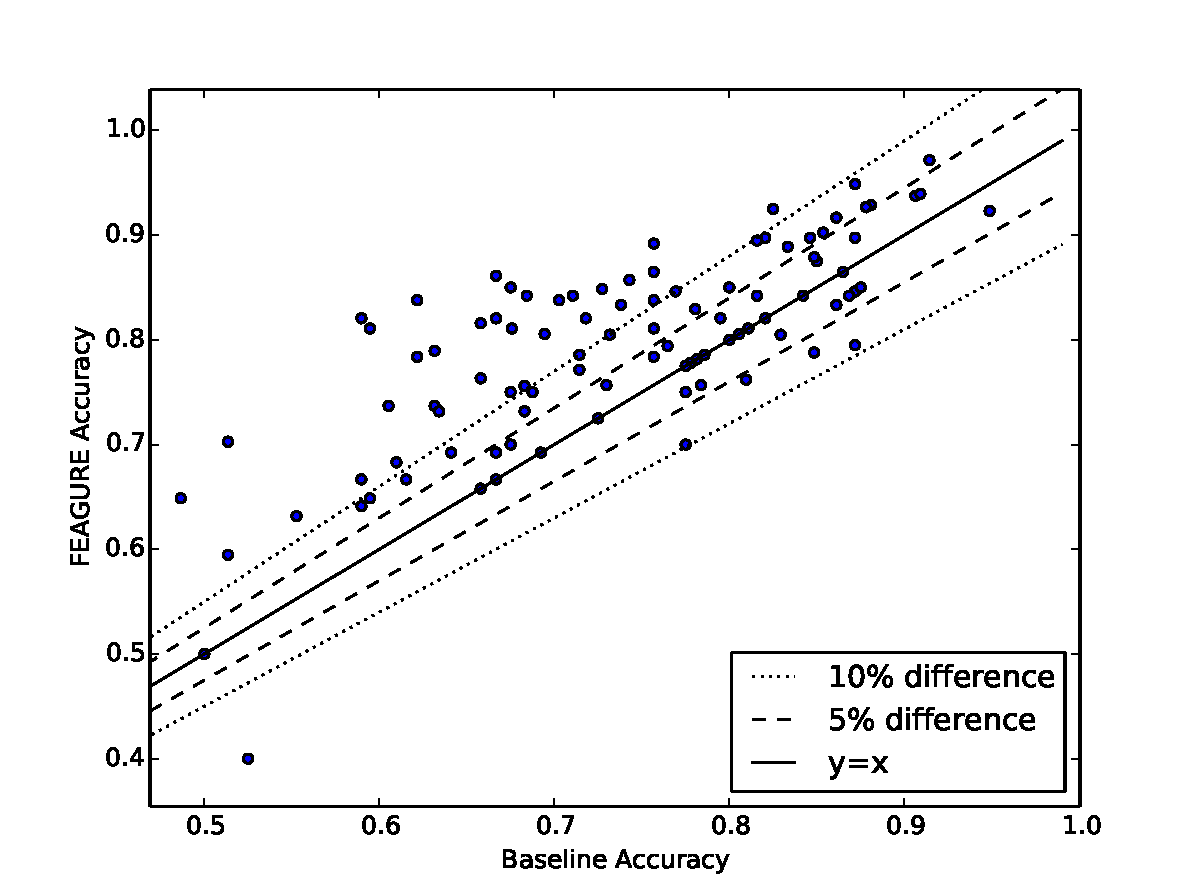
\includegraphics[width=0.7\linewidth]{svm_full}
%	\caption{Accuracy of
%		baseline approach compared to single activation of \emph{FEAGURE} (SVM). Each point represents a dataset. The dotted lines represent a 5 and 10 percent difference in accuracy}
%	\label{fig:svm_base_lvl1}
%\end{figure}

\begin{figure}
	\centering
	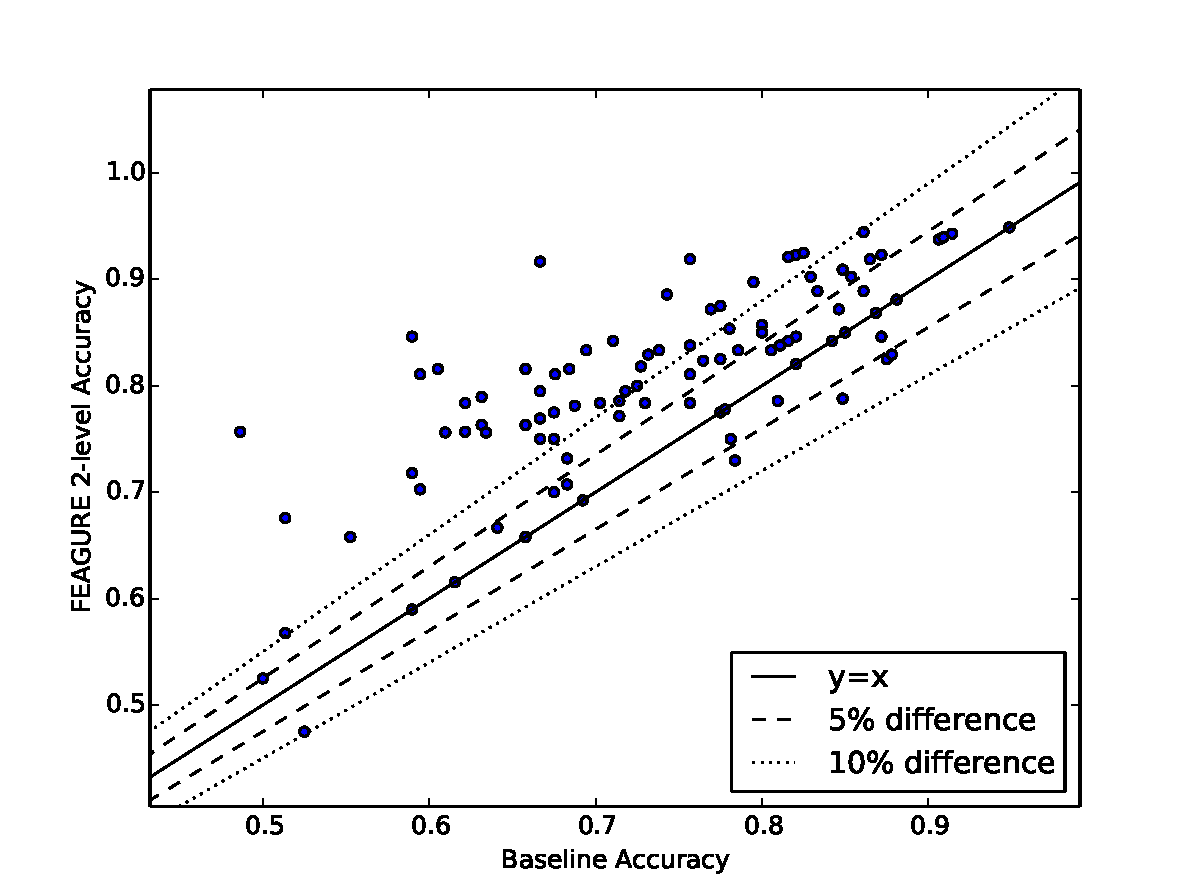
\includegraphics[width=0.7\linewidth]{svm_full_lvl2}
	\caption{Accuracy of
		baseline approach compared to two-level activation of \emph{FEAGURE} (SVM). Each point represents a dataset. The dotted lines represent a 5 and 10 percent difference in accuracy}
	\label{fig:svm_base_lvl2}
\end{figure}

The results show a strong trend of improvement, with high ($>10\%$) improvement being common.
%For a single activation, we see 15 datasets where no change in accuracy is observed. This is due to a low number of generated features, as relatively few entities have been extracted. For 13 datasets, we see a degrade in accuracy, 5 of which showing  a degrade of over $5\%$.
%For a two-level activation, 12 datasets show no change in accuracy, and only 8 datasets show a degrade in accuracy, with the same 5 datasets showing notable degrade.

We see that for 8 of the datasets, there is a degrade in accuracy. This degrade in accuracy can be explained due to a combination of several factors:
\begin{itemize}
	\item Errors in the entity extraction process cause potential entity candidates to remain hidden.%, thus denying their use in later stages.
	\item Errors in the entity linking process may lead to the creation of mistaken entities and thus features. %For instance, the word ``One" may be interpreted as the entity ``One (Metallica song)".
	\item Over-fitting within the feature generation algorithm may create features that appear to have high information gain while generalizing poorly to test data.
\end{itemize} 

In their paper on TechTC-100, \cite{gabrilovich2004text} define a metric known as Maximal Achievable Accuracy (MAA). This criterion attempts to define the difficulty of the induction problem by finding the maximal accuracy among three induction algorithms (SVM, K-NN and CART).
Intuitively, a dataset with low MAA can be considered harder than one with a high MAA.%, since a known induction algorithm can achieve a higher accuracy for the dataset with higher MAA.
%Figure \ref{fig:25best} shows the 25 hardest datasets in TechTC-100, in terms of the MAA criterion. We call this dataset collection ``TechTC-25MAA". 
Table \ref{table:acc} also shows the accuracies for the 25 hardest datasets in TechTC-100, in terms of the MAA criterion. We call this dataset collection ``TechTC-25MAA". %The table uses the same terminology for significance and best results as before.
%We see that for 3 of the datasets in TechTC-25MAA, there is no change in accuracy, either due to the lack of features or due to lack of contribution in the final classifier.
%For 2 of the 25 datasets, we see a minor improvement in accuracy. For the remaining 17 of them, we see an improvement of $5\%$ or above, with the highest being over $20\%$.
%Of the 25 datasets, 3 show a degrade in accuracy, with 2 of them being a serious degrade. 

These results show a much more pronounced accuracy increase, and illustrate that we can, in general, rely on \emph{FEAGURE} to yield positive features for difficult classification problems.

%\begin{table}[!h]
%	\centering
%	\caption{Average accuracy over 25 hardest datasets in terms of MAA. The columns specify feature generation approach, with baseline being no feature generation. The rows specify the induction algorithm used on the generated features for evaluation. Best results are marked in bold.}
%	\label{table:acc_maa}
%	\begin{tabular}{|l | l || l | l | l| l|}
%		\hline
%		Dataset & Classifier & Baseline   & Expander-FG & FEAGURE   & FEAGURE 2-level    \\ \hline
		
		%\multirow{3}{*}{TechTC-25MAA} & KNN & 0.524 & 0.723 ($p<0.001$) & \textbf{0.803 ($p<0.001$)} & 0.795 ($p<0.001$)  \\ \cline{2-6}
		
		% & SVM  & 0.751 & 0.815 ($p<0.001$)    & 0.817 ($p<0.001$)    & \textbf{0.829 ($p<0.001$)} \\ \cline{2-6}
		
		% & CART  & 0.82 & 0.839   & 0.837   & \textbf{0.849 ($p<0.05$)}  \\
		
		%\specialrule{.15em}{.05em}{.01em}
		
%	\end{tabular}
%\end{table}

%\begin{figure}
%	\centering
%	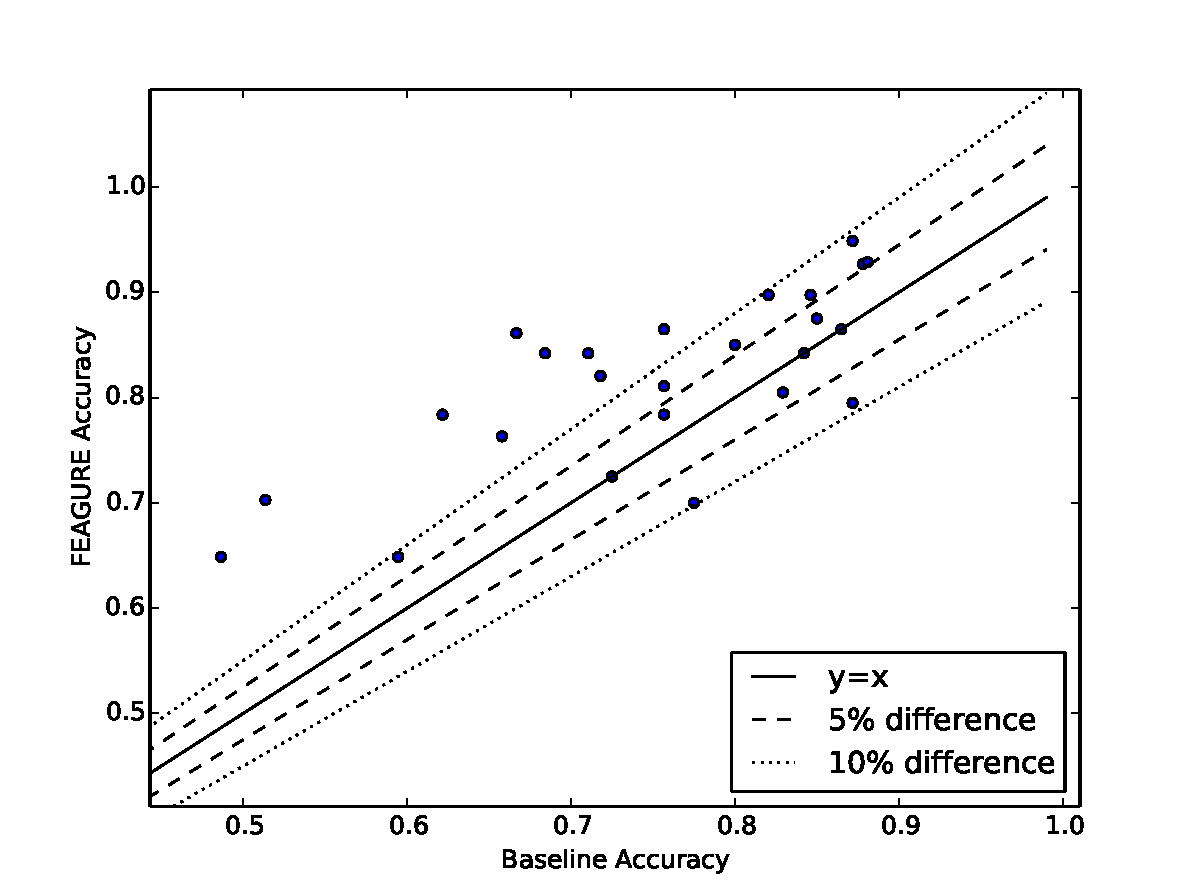
\includegraphics[width=0.8\linewidth]{25best}
%	\caption{Accuracy of
%		baseline approach compared to single-level activation of \emph{FEAGURE} (SVM). Displayed are the 25 hardest datasets (meaning they have the lowest MAA)}
%	\label{fig:25best}
%\end{figure}

%In order to better understand the difference in results, 
%We also looked at the 25 datasets with highest number average entities per text. We named this new dataset collection TechEC-25.%, meaning Technion Repository of Entity Categorization Datasets.
%Table \ref{table:acc} compares the two datasets. We see that the results for TechEC-25 are much more pronounced than those for TechTC-100. This result indicates that better entity linking, which results in more correct entities per text, is potentially very beneficial to \emph{FEAGURE}'s performance.

%\begin{table}[]
%	\centering
%	\caption{Average accuracy over all datasets. The columns specify feature generation approach, with baseline being no feature generation. The rows specify the induction algorithm used on the generated features for evaluation.}
%	\label{table:acc_ec25}
%	\begin{tabular}{|l | l || l | l | l| l|}
%		\hline
%		Dataset & Classifier & Baseline   & Expander-FG & FEAGURE   & FEAGURE 2-level    \\ \hline
%		\multirow{3}{*}{TechEC-25} & KNN  & 0.539 & 0.72 ($p<0.001$) & 0.777 ($p<0.001$)  & \textbf{0.781 ($p<0.001$)} \\ \cline{2-6}
%		& SVM  & 0.762 & 0.788  & \textbf{0.82 ($p<0.001$)}    & 0.817 ($p<0.05$) \\ \cline{2-6}
		
%		& CART  & 0.81 & 0.833   & 0.836 ($p<0.05$)    & \textbf{0.847 ($p<0.05$)} \\
		
		%\specialrule{.15em}{.05em}{.01em} % \hline
		
		%\multirow{3}{*}{TechTC-100} & KNN & 0.531 & 0.702 ($p<0.001$) & 0.772 ($p<0.001$) & \textbf{0.775 ($p<0.001$)}  \\ \cline{2-6}
%		& SVM  & 0.739 & 0.782 ($p<0.001$)    & 0.796 ($p<0.001$)    & \textbf{0.807 ($p<0.001$)} \\ \cline{2-6}
		
%		& CART  & 0.81 & 0.815   & 0.814   & \textbf{0.825 ($p<0.05$)}  \\
		
%		\specialrule{.15em}{.05em}{.01em}
		
%	\end{tabular}
%\end{table}

\subsection{Effect of recursive problem classifier on \emph{FEAGURE}}

As we have discussed in section \ref{algorithm_section}, \emph{FEAGURE} creates a generic learning problem as part of its execution. In this section, we will test the effects of using various induction algorithms on these recursive problems. We have chosen to try both K-NN and SVM.%, with the following parameters: For K-NN, we used $K=3$. For SVM we used $C=10$, with both Linear and a Radial Basis Function (RBF) kernels.

We note that this choice is orthogonal to that of the induction algorithm used to evaluate the generated features.

Table \ref{table:acc-nontree} shows the accuracies achieved by using these induction algorithms. We see that in general, with the exception of K-NN (all references are to the external induction algorithm), the results are slightly poorer than those achieved by our approach as well as the \emph{Expander-FG} algorithm. Despite this, however,  many of these results do show an improvement over the baseline.
%Of particular note are the results for K-NN classifiers for both TechTC-100 and OHSUMED. In both cases, K-NN classifiers showed a marked improvement over the baseline approach. This can be attributed to the fact that unlike \emph{Expander-FG} and our results when using decision trees as inner classifiers, the number of generated features for these approaches is much smaller, thus allowing each feature to have a greater effect.
The most noteworthy of the results shown in table \ref{table:acc-nontree} are those referring to K-NN for the OHSUMED dataset. Here we see, for the first time, a significant improvement over the baseline approach.

\begin{table*}[!th]
	\centering
	\caption{Average accuracy over all datasets. The columns specify the induction algorithm used in \emph{FEAGURE} (SVM with linear or RBF kernel, K-NN). The rows specify the induction algorithm used on the generated features for evaluation. Entries marked with * show a statistically significant p-value over the baseline accuracy}
	\label{table:acc-nontree}
	\centering
	\begin{tabular}{|l | l || l || l | l| l|l|}
		\hline
		Dataset & Classifier  & Baseline & Expander-FG & Tree  & RBF SVM & 5-NN    \\ \hline
		
	\multirow{3}{*}{OHSUMED} & KNN  & 0.777 & 0.756 & 0.769 & \textbf{0.795*}   & 0.771 \\ \cline{2-7}
		& SVM  & 0.797 & 0.804 & \textbf{0.816*}   & 0.796    & 0.788 \\ \cline{2-7}
		
		& CART  & 0.806 & \textbf{0.814} & 0.809   & 0.791    & 0.787 \\
		
		\specialrule{.15em}{.05em}{.01em} % \hline
		
		\multirow{3}{*}{TechTC-100} & KNN & 0.531 & 0.702* & \textbf{0.772*} & 0.689*   & 0.705*\\ \cline{2-7}
		& SVM   & 0.739 & 0.782* & \textbf{0.796*}  & 0.774*   & 0.774* \\ \cline{2-7}
		
		& CART & 0.81 & \textbf{0.815} & 0.814   & 0.81    & 0.79 \\
		
		\specialrule{.15em}{.05em}{.01em} % \hline
		
		%\multirow{3}{*}{TechTC-25H} & KNN & 0.524 & 0.723* & \textbf{0.803*} & 0.744* & 0.7239*   & 0.724*\\ \cline{2-8}
		%& SVM   & 0.751 & 0.815* & \textbf{0.817*} & 0.794*  & 0.799*   & 0.782* \\ \cline{2-8}
		
		%& CART & 0.82 & \textbf{0.839} & 0.837 & 0.786   & 0.799    & 0.801 \\
		
		%\specialrule{.15em}{.05em}{.01em} % \hline
		
	\end{tabular}
\end{table*}

\section{Related Work}

Feature generation approaches were found useful for a wide variety of learning problems \citep{markovitch2002feature,ragavan1993complex,utgo1991linear}.
These feature generation approaches search for new features that better represent the target concept than existing features. To that end, there are three major approaches for feature generation: tailored approaches, combinational techniques and methods utilizing external knowledge.
Tailored approaches \citep{hirsh1994bootstrapping} are designed for specific problem domains and rely on domain-specific background knowledge. %for feature construction. 
%One such example is the bootstrapping algorithm \cite{hirsh1994bootstrapping}, which was designed for the domain of molecular biology. The algorithm represents features as nucleotides sequences
%whose structure is determined by existing background knowledge. The algorithm uses an initial set of feature sequences, produced by human experts, and uses a domain-specific set of operators to alter them into new sequence features. 
Such special-purpose algorithms% may be effectively tailored for a given domain, but 
 have proven difficult to generalize to other domains and problems

Combinational feature generation techniques aim to locate more descriptive features by combining existing features in various ways, without regards to the specific problem domain. %The LDMT algorithm \cite{utgo1991linear}, for example, performs feature construction in the course of building a decision-tree classifier. At each created tree node, the algorithm constructs a hyperplane feature through linear combinations of existing features in a way likely to produce concise, relevant hyperplanes. The FICUS algorithm \cite{markovitch2002feature} describes a general architecture for all combinational feature generation techniques, based on an a feature space specification: a grammar describing the problem domain.

Another major class of combinational feature generation approaches is that of \emph{Deep Learning} \citep{plotz2011featurefull,kim2013deepfull}. Deep learning techniques seek to create features through complex combinations of existing features, using a deep structure of linear and non-linear functions.
%Doing so allows for a wide variety of possible combinational features.
%This technique bears some similarities to our approach, in that it allows for the creation of complex features. 
Unlike deep learning methods, our approach utilizes external knowledge to further improve the generated features. Furthermore, our use of induction algorithms allows for a more generic combination of features.

%\subsection{Knowledge based feature generation}

In contrast to combinational approaches, some feature generation algorithms, including \emph{FEAGURE}, seek to inject additional knowledge into the existing learning problem. These approaches seek to do so almost exclusively through the use of relational data. 
%Within this wide family of knowledge-based approaches, we can see a clear distinction between unsupervised and supervised approaches.
%Unsupervised knowledge-based feature generation techniques aim to incorporate additional knowledge from external sources without consideration to the labels supplied by a given training set. They do so in several differing ways:
%Of these approaches, several are unsupervised:
%\begin{itemize}
	%\item
	
	 Concept based approaches such as ESA \citep{gabrilovich2009wikipediafull} present a method for generating features that are based on semantic concepts. %These approaches rely on complex techniques to create a mapping between existing data and the semantic concepts that serve as external knowledge. This mapping is then used on the given problem, enriching the data with external concepts that can be used as features. 
	ESA, for example, maps texts to Wikipedia pages that are used as concepts.
	%\item
	
	 Propositionalization \citep{kramer2000bottom} approaches are a class of feature generation algorithms that rely on relational data to serve as external knowledge. They operate by using a combination of operators in order to create first-order logic predicates connecting existing data and relational knowledge. 
	\cite{cheng2011automatedfull} devised a generic propositionalization framework  using linked data via relation-based queries. % and offer an insight into using taxonomy-based features by creating features that list the taxonomic class relationships of a given entity.
	The \emph{Expander-FG} algorithm described in section \ref{shallow_section} is another example of propositionalization algorithms.
	%\item
	
	 Data mining approaches such as FeGeLOD \citep{paulheim2012unsupervisedfull} aim to directly utilize linked data in order to automatically enrich existing data. % yielding additional information on existing entities within the data. 
	FeGeLOD uses feature values as entities and adds related knowledge to the example. %, thus creating additional features for that example. FeGeLOD then employs feature selection to filter out poor, non-representative features. 
	Our approach can be seen as a continuation of this approach, as we keep the notions of feature enrichment and feature selection, but utilize a supervised enrichment process rather than an unsupervised one.
%\end{itemize}

%These knowledge-based techniques serve as a powerful tool for feature generation based on knowledge. Despite this fact, the unsupervised nature of these approaches tends to lead to a shallow exploration of the knowledge base, as deep unguided search is computationally expensive, and leads to a potentially large number of features. %As a result of this, many of these approaches rely on feature selection to filter out irrelevant features.

Unlike unsupervised approaches, some methods, \emph{FEAGURE} included, seek to utilize a labelled training set in order to perform a more guided search through the space of possible features based on external knowledge. 
Most of these techniques can trace their source to \emph{Inductive Logic Programming (ILP)} \citep{quinlan1990learning}, a supervised approach that induces a set of first-order logical formulae with the purpose of achieving a good separation of the given training set. 
%ILP methods do so by starting from single relation formulae and adding additional relational constraints using the knowledge base, until formulae that separate the training set into positive and negative examples are found. To that end, these approaches make use of an operator known as a refinement operator. When applied on a relational formula, a refinement creates a more specialized case of that formula. For example, given the logical formula $BornIn(X,Y)$, where $X$ is a person and $Y$ is a city, one possible refinement is the formula $BornIn(X,Y)\land CapitalOf(Y,Z)$, where $Z$ is a country. The result is a logical formula that considers a more specific case. Additionally, we can look at a refinement that restricts by a constant, turning $BornIn(X,Y)$ into, for example, $BornIn(X, \mbox{{United States}})$.This refinement process continues until a sufficient set of consistent formulas is found.

%An algorithm suggested by \cite{terziev2011feature} shows an interesting approach to supervised feature generation. In his paper, \cite{terziev2011feature} suggests a decision tree based approach, where in each node of the tree, an expansion of features is done similarly to FeGeLOD, with a criteria based on entropy used to decide whether further expansion is required. This technique bears several similarities to the approach of \emph{Deep-FEAGURE} (Algorithm \ref{code-tree-thing}). Unlike Deep \emph{FEAGURE}, the feature expansion process is unsupervised, and the resulting feature must be a decision tree, restricting the generality of the approach.

\emph{Upgrade} methods such as ICL \citep{van2001upgrade} and SGLR \citep{popescul200716} can be seen as the supervised equivalent of propositionalization methods. Instead of creating first-order predicates a-priori, feature generation is performed during the training phase, allowing for complex features to be considered. % thanks to a more structured search process that utilizes feature selection based on the target concept.
While upgrade approaches bear some similarities to our approach, there are several critical differences, the key of which being the ability to more easily locate complex features through the use of existing induction algorithms. 

%Another type of supervised, knowledge-based, feature generation approaches is \emph{Relational Learning} techniques. These techniques are designed to utilize relational databases and expand their knowledge. One such technique is that of View Learning \cite{davis2005view}. View learning generates new relational tables from the existing relational knowledge, based on labelled data.
%It does so by applying ILP on relational data to construct new, simple, relational tables, then using a Bayesian network induction algorithm, learns ways in which these relations can be combined more effectively into a single, more complex table.
%This approach bears similarity to our approach in that it can effectively utilize background knowledge to draw conclusions using the combination of labelled data and background knowledge. Unlike our approach, these views attempt to fit new knowledge to existing examples, whereas our approach re-frames the learning problem within a new context.

%Kernel-based knowledge injection techniques aim to make use of powerful machine learning algorithms such as SVM and Deep-learning techniques by decoupling the knowledge base from the induction algorithm. This is done through the use of a kernel function that acts as a similarity function between examples in the problem domain. An example of this approach can be seen in the work of \cite{losch2012graph}, which attempts to learn graph kernels within the relational domain. This creates strong kernel functions that look at the neighbourhood of an entity in search of similarities between entities. This approach bears some similarity to our own in that it can locate complex relationships, but they fundamentally differs in their approach. Kernel methods attempt to create a filter through which entity similarity can be measured. In our approach, we attempt to locate the target concept through the use of different domains. This distinction is especially relevant to classification tasks, where many possible domains can apply for each example, and similarity may be difficult to find when considering the entire example set.
%TODO: mby

%\emph{FEAGURE} itself is a supervised knowledge-based feature generation approach. It focuses on creation of recursive induction problems, in a manner reminiscent of view learning. This construction allows for a complex exploration of features, which can then be combined in general ways using existing induction methods, in a manner resembling combinational feature generation approaches.
%The features of recursive learning problems created by \emph{FEAGURE} during the feature generation process are similar to those constructed by ILP, relying on a technique that resembles refinement operators. 

%\subsection{Knowledge bases and entity linking}

%In recent years, we have seen a massive surge in the popularity of relational knowledge bases, starting from the Semantic Web project \cite{bizer2009linkedfull}, through Wikidata \cite{vrandevcic2014wikidata} and more recently, the Google knowledge graph \cite{pelikanova2014google}.

%With the increased availability of such knowledge bases, several methods have been devised to make use of them, including several approaches discussed above.
%In order to make use of these knowledge bases, one of two conditions must be true:
%One possibility is that the problem at hand is already one whose problem domain is entities, such as link prediction \cite{popescul2003statistical2,getoor2005link} and collective classification algorithms \cite{raghavan2004exploration,kajdanowicz2013collectiveaa}. These algorithms assume an existing knowledge base, and attempt to operate within it by either adding links (or relational facts) in the case of the first or by propagating classifications in that of the second.

%The other option is to map objects in the problem domain to entities in some way.
%To that end, there exist many methods to map objects to entities, ranging from various Entity Recognition \cite{nadeau2007survey} methods, through enriching approaches such as ESA \cite{gabrilovich2009wikipediafull}, to Entity Linking \cite{rao2013entity} and Wikification \cite{bunescu2006using,cheng2013relational}. 
%All of the above approaches attempt to map in a variety of ways.
%We have already discussed ESA previously, but we note that it has been used to link texts to Wikipedia concepts that can be used as entities in many modern relational knowledge bases.

%Most Entity Recognition approaches rely on statistical methods combined with linguistic grammar. Through these methods, part-of-speech can be recognized, and likely candidates for entities can be found and cross-referenced with the knowledge base. A better way to link the extracted entities with the ones in the knowledge base is Entity linking. This process seeks to enhance entity recognition by better linking the entities through candidate selection and ranking.
%Another approach to this problem is called Wikification. This method seeks to unify the two separate processes of recognition and linking. Similarly to enriching approaches such as ESA, these approaches seek to link words with Wikipedia concepts. 

%anything else? still a bit short


\section{Conclusions}
%finishing up and summary

In this paper, we presented and evaluated \emph{FEAGURE}, a supervised, knowledge-based feature generation algorithm. Our approach is based around the concept of injecting traditional induction algorithms with external knowledge. %through the use of features constructed in a supervised manner based on the target concept. 
The algorithm does so through the creation of recursive learning problems based on existing features and the knowledge base, that is then given as input to an induction algorithm. The output of this process is a classifier that is then turned into a feature for the original problem.

%In section \ref{formal}, we discussed the feature generation setting, looked at the ways by which an unsupervised approach can be used for feature generation given a complex relational knowledge base, and explained our approach in detail.

%In section \ref{text-feagure}, we considered the domain of text categorization as a possible problem for which our approach can be applied, through the use of the bag-of-entities approach. We proceeded to empirically evaluate of our approach on the text categorization learning problem.
%Empirical evaluation of our approach confirmed that complex knowledge-based feature generation significantly improves classifier accuracy. Experiments on the TechTC-100 dataset show an improvement over a wide range of problems of varying difficulty, with problems considered difficult yielding a very high improvement overall.

The main strength of our approach is its ability to use existing induction approaches in a meaningful way on the knowledge base, allowing for the creation of complex features. These features can then be used by any induction algorithm, giving us a powerful, generic approach.

One limitation of our approach is that even more so than unsupervised feature generation algorithms,  we are dependant on a correct link between feature values and entities within the knowledge base. %Mistaken links can lead to incorrect features within the constructed learning problems that may cause the classifier learned to represent a false hypothesis. 

%While we focused on applying this approach to text categorization problems, it is important to note that it is applicable to any classification problem where entities can be extracted from feature values, such as drug names, cities and so on. 

%% The file named.bst is a bibliography style file for BibTeX 0.99c
\clearpage
\bibliographystyle{named}
\bibliography{document}

\end{document}

